\documentclass{llncs}
\usepackage[a4paper,hmargin=1in,vmargin=1.25in]{geometry}

\usepackage{llncsdoc}
\usepackage[T1]{fontenc}
\usepackage[english]{babel}
\usepackage[utf8]{inputenc}
\usepackage{listings}
\usepackage{graphicx}
\usepackage{verbatim}
\usepackage{hyperref}           % PDF with links
\usepackage{fancyvrb}           % SaveVerbatim
\usepackage{amsmath}
\usepackage{amssymb}

\begin{document}
\sloppy

\pagestyle{myheadings}
\markboth{Laser Point}{Muzzley}

\title{Laser Pointer}
\subtitle{Using Android to simulate a Laser Pointer}
\author{Rui Gonçalo
        \\{\scriptsize \texttt{ruimiguelgoncalo@gmail.com}}
       }
\date{\today}
\maketitle


\begin{abstract}
Some notes about the development of a Laser Pointer using Android, Node.js and socket.io.
\end{abstract}

%-----------------------------------------------------------------------
\section{Android app}

The Android app related files are store at the \texttt{Laser} folder in the root of the repository. Note that it was used the Eclipse IDE to develop the Android app. Briefly, the app uses the \textbf{accelerometer} sensor to get the 3-axis coordinate system values x, y and z, corresponding to the device's movements. These values are sent to the remove server using the \textbf{socket.io} library.

\subsection{User Interface}

\begin{figure}[h]
 \centering
 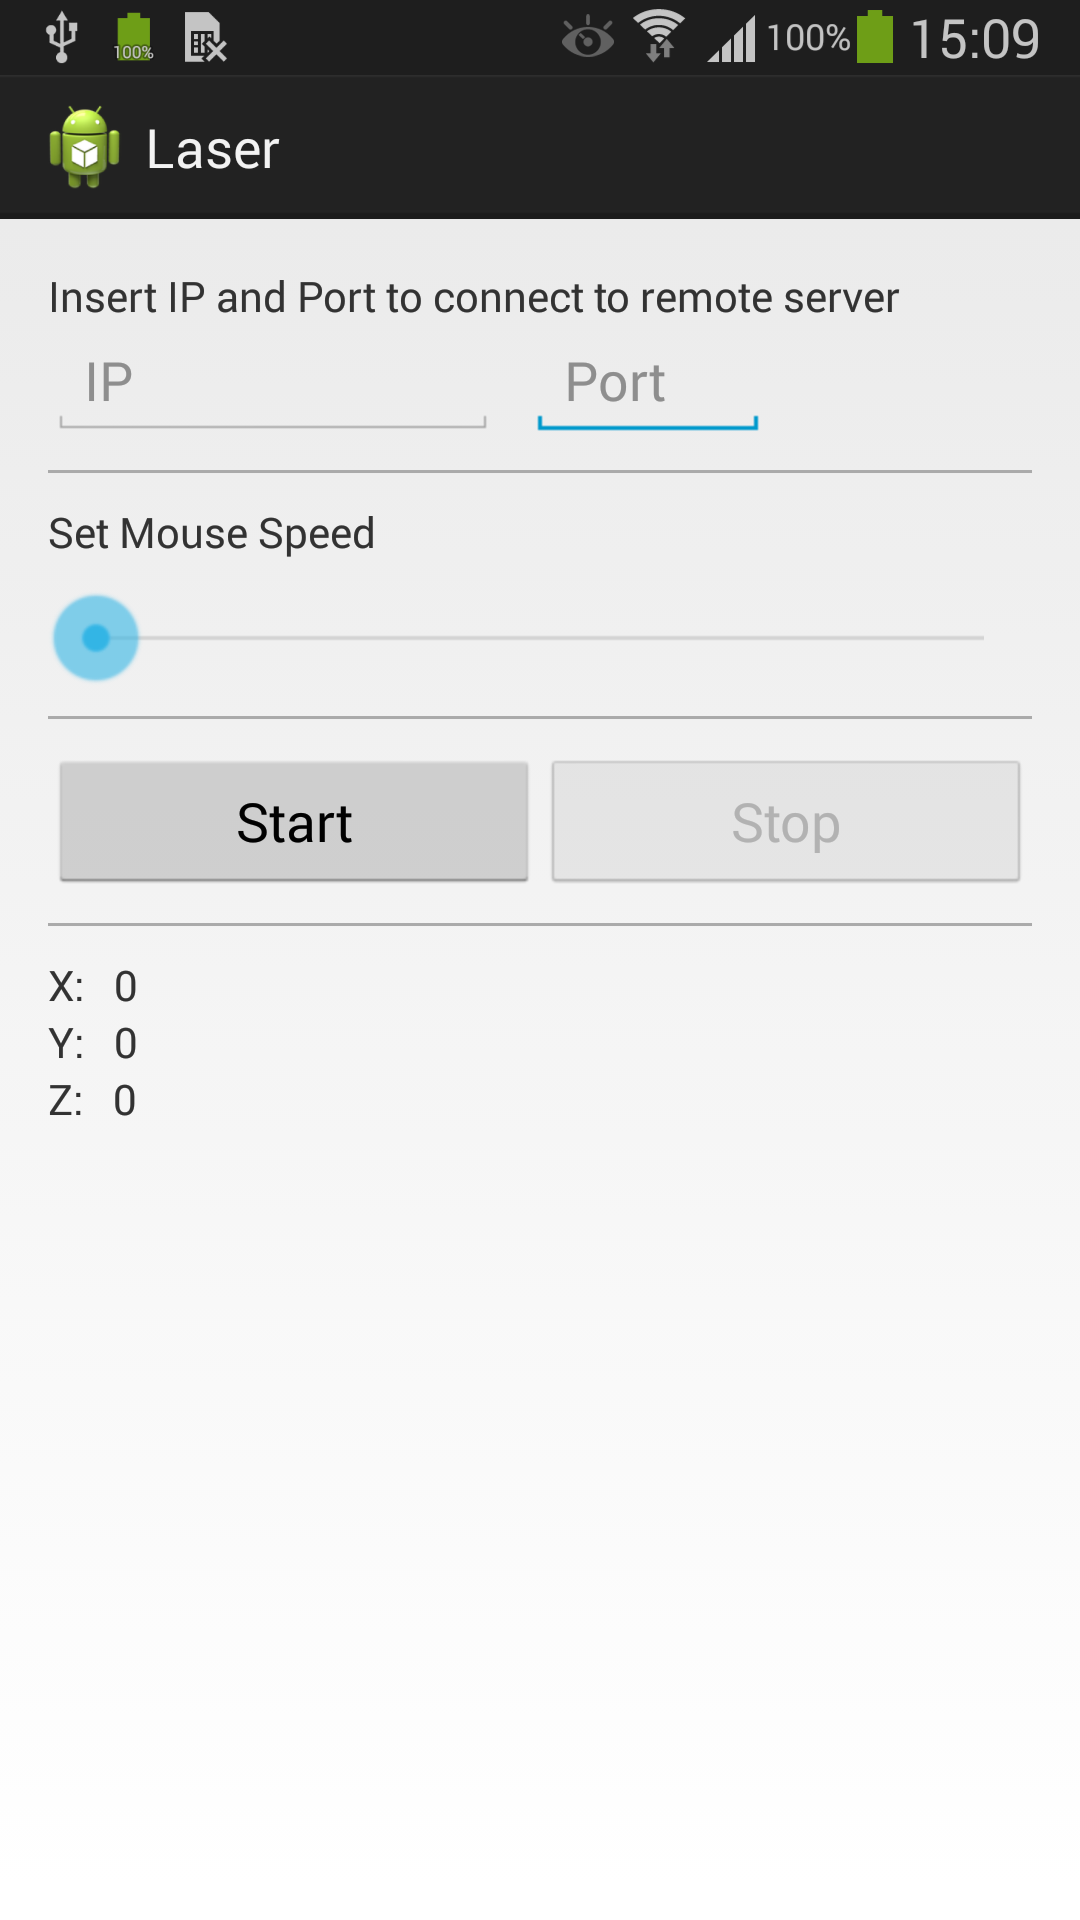
\includegraphics[scale=0.18]{figures/screenshot.png}
 \caption{User Interface}
 \label{fig:ui}
\end{figure}

\autoref{fig:ui} shows the User Interface. The first elements are used to insert the IP address (xxx.xxx.xxx.xxx) and port of the remote server. Note that the port must be \textbf{33001}, because it is the one defined on the server. However, the port is introduced by an \textit{EditText} because if the server changes the port value, the app do not need to be changed.
\\

\noindent If the user do not fill in both \textit{EditText} boxes the sensor do not start running. The string values of each text are not being validated, but this feature is marked as future work.
\\

\noindent After inserting the remote address and port, the user must provide a mouse speed value using the \textit{SeekBar}. This element is defined to have a maximum value of 20, which means that the range is between 0 and 20. If the speed value is equal to 0, the sensor will not start running.
\\

\noindent Below, there are two \textit{Buttons} that start and stop (pause) the sensor. This way, the user has a satisfactory control over the sensor, being able to start and stop it whenever he desires.
\\

\noindent At last, the sensor values are displayed below the buttons as a debug feature. In fact, one of the major difficulties was to convert these values into coherent coordinates to send to the remote server.
\\

\noindent Since it is not functional to have the screen rotating while the device is moving, it was blocked the portrait orientation by adding \texttt{android:screenOrientation="portrait"} on the Manifest file.

\subsection{Accelerometer Values}

As mentioned above, it was not easy to convert the sensor values. At the moment, the app is reading the \texttt{event.values} variable and applying both a low-pass filter and a high-pass filter that are provided on the Android motion sensors page\footnote{http://developer.android.com/guide/topics/sensors/sensors\_motion.html}. The mouse sensitivity is provided through the \texttt{speed} variable that is used in the high-pass filter. According to its value (0-20) the pointer moves slower or faster.

\subsection{Socket.io}

In order to connect to the remote server, it was used the \texttt{socket.io-java-client} library available on GitHub\footnote{https://github.com/Gottox/socket.io-java-client}. A simple tutorial\footnote{http://nkzawa.tumblr.com/post/46850605422/connecting-to-a-socket-io-server-from-android} was used to learn the main methods. It is established a new connection every time the user clicks on the start button.

%-----------------------------------------------------------------------
\section{Server}

It was used \textit{Node.js} to implement the server that receives the Android app data. The files related to the server are placed at the \texttt{laser-server} folder in the root of the repository. These files were created using the \textit{Express} framework.
\\

\noindent The main file is the \texttt{app.js} that implements the server. It uses the \texttt{socket.io} library to create a socket server that is listening on port \textbf{33001}. The following code snippet states the server behavior:

\begin{lstlisting}
io.sockets.on('connection', function(socket) {
  socket.on('echo', function(data) {
     socket.broadcast.emit('position',data);
  });
});
\end{lstlisting}

Whenever the socket receives a \texttt{connection} event it waits for the \texttt{echo} event and broadcasts the \texttt{data} object. The \texttt{connection} event is used to connect to the client (this client is the browser) and the \texttt{echo} event is used to connect to the Android app.

%-----------------------------------------------------------------------
\section{Client}

The files related to the client are placed at the same folder as the server. The technology used to draw an HTML element in real-time was \textit{AngularJS}. The main files are \texttt{views/index.ejs} and \texttt{public/javascript/pointer.js}. The first file contains HTML elements to draw the container and the pointer. The last file handles the socket connection in order to get the data sent by the Android app.
\\

\noindent The pointer moves in the container by being constantly updated its \texttt{margin} values within the \texttt{style} attribute, as presented in the following code snippet:

\begin{lstlisting}
<div ng-app="pointer">
  <div ng-controller="pointer">
    {{coor}} {{width}} {{height}}
     <div class="img-circle" 
         style="margin-left:{{width}}px; 
               margin-top:{{height}}px; 
               width:{{size}}px; height:{{size}}px;">
     </div>
  </div>
</div>
\end{lstlisting}

The \texttt{coor}, \texttt{width} and \texttt{height} variables are defined and updated in the \texttt{pointer.js}, explained in the following section.

\subsection{Moving the pointer}

The following code snippet shows the function responsible for translating the Android app values into pointer movements on the HTML page:

\begin{lstlisting}
pointer.controller('pointerctrl', ['$scope','socket', function($scope, socket) {
    $scope.height =$(window).height()/2;
    $scope.width = $(window).width()/2;
    $scope.size = 20;
    socket.on('position', function (data) {
      $scope.coor = data;

      $scope.height -= parseFloat(data.y);
      $scope.width -= parseFloat(data.x);

      var h_aux = $scope.height;
      var w_aux = $scope.width;

      if( h_aux < 0)
        $scope.height = 0;

      if( h_aux > $(window).height())
        $scope.height = $(window).height();

      if( w_aux < 0)
        $scope.width = 0;

      if( w_aux > $(window).width())
        $scope.width = $(window).width();

      //$scope.size += parseFloat(data.z);
    });
}]);
\end{lstlisting}

At first, the pointer is placed in the center of the page, by calculating the width and height of the window. It is defined a 20px size to the pointer. The Android app values are inspected using \texttt{data.x} and \texttt{data.y}. By parsing these values and subtract the window's height and with by them it is possible to get a \textbf{very irregular} movement of the pointer that corresponds to the Android device's motion.
\\

\noindent In order to get the pointer inside the container, it is being checked the window's height and width so that the margin values cannot turn into negatives or greater than the window's borders.

\end{document}
